\documentclass[]{standalone}
\usepackage{tikz}
\usepackage{pgffor}

\standaloneenv{tikzpicture}

\usetikzlibrary{arrows}

\begin{document}
	
	
	%% output-name: spanning_trees_01
    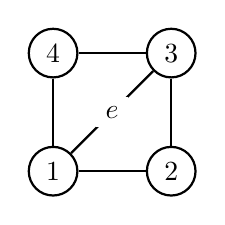
\begin{tikzpicture}[node distance={15mm}, thick, main/.style = {draw, circle}]
        \centering
        \node[main] (1)              {1}; 
        \node[main] (2) [right of=1] {2};
        \node[main] (3) [above of=2] {3}; 
        \node[main] (4) [left of=3] {4};
        \draw  (1) -- (2) ;  
        \draw  (1) -- (3) node [midway, fill=white] {$e$};  
        \draw  (1) edge (4); 
        \draw  (4) edge (3); 
        \draw  (2) edge (3); 
    \end{tikzpicture}

    %% output-name: spanning_trees_02
    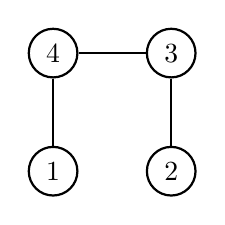
\begin{tikzpicture}[node distance={15mm}, thick, main/.style = {draw, circle}]
        \centering
        \node[main] (1)              {1}; 
        \node[main] (2) [right of=1] {2};
        \node[main] (3) [above of=2] {3}; 
        \node[main] (4) [left of=3] {4};
        \draw  (1) edge (4); 
        \draw  (4) edge (3); 
        \draw  (2) edge (3); 
    \end{tikzpicture}
    
    %% output-name: spanning_trees_03
    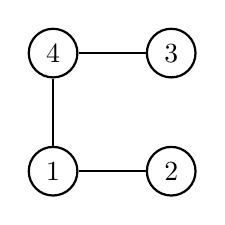
\begin{tikzpicture}[node distance={15mm}, thick, main/.style = {draw, circle}]
        \centering
        \node[main] (1)              {1}; 
        \node[main] (2) [right of=1] {2};
        \node[main] (3) [above of=2] {3}; 
        \node[main] (4) [left of=3] {4};
        \draw  (1) edge (4); 
        \draw  (4) edge (3); 
        \draw  (2) edge (1); 
    \end{tikzpicture}
    
    %% output-name: spanning_trees_04
    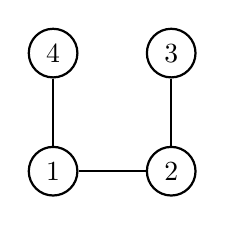
\begin{tikzpicture}[node distance={15mm}, thick, main/.style = {draw, circle}]
        \centering
        \node[main] (1)              {1}; 
        \node[main] (2) [right of=1] {2};
        \node[main] (3) [above of=2] {3}; 
        \node[main] (4) [left of=3] {4};
        \draw  (1) edge (4); 
        \draw  (2) edge (1); 
        \draw  (2) edge (3); 
    \end{tikzpicture}
    
    %% output-name: spanning_trees_05
    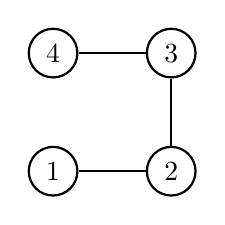
\begin{tikzpicture}[node distance={15mm}, thick, main/.style = {draw, circle}]
        \centering
        \node[main] (1)              {1}; 
        \node[main] (2) [right of=1] {2};
        \node[main] (3) [above of=2] {3}; 
        \node[main] (4) [left of=3] {4};
        \draw  (3) edge (4); 
        \draw  (2) edge (1); 
        \draw  (2) edge (3); 
    \end{tikzpicture}

    %% output-name: spanning_trees_06
    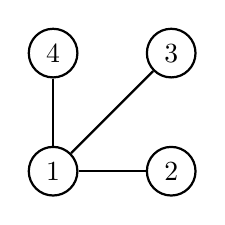
\begin{tikzpicture}[node distance={15mm}, thick, main/.style = {draw, circle}]
        \centering
        \node[main] (1)              {1}; 
        \node[main] (2) [right of=1] {2};
        \node[main] (3) [above of=2] {3}; 
        \node[main] (4) [left of=3] {4};
        \draw  (1) edge (2); 
        \draw  (1) edge (3); 
        \draw  (1) edge (4); 
    \end{tikzpicture}
    
    %% output-name: spanning_trees_07
    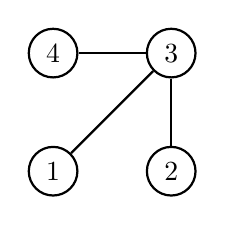
\begin{tikzpicture}[node distance={15mm}, thick, main/.style = {draw, circle}]
        \centering
        \node[main] (1)              {1}; 
        \node[main] (2) [right of=1] {2};
        \node[main] (3) [above of=2] {3}; 
        \node[main] (4) [left of=3] {4};
        \draw  (1) edge (3); 
        \draw  (2) edge (3); 
        \draw  (3) edge (4); 
    \end{tikzpicture}
    
    %% output-name: spanning_trees_08
    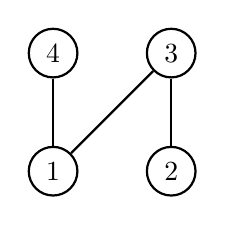
\begin{tikzpicture}[node distance={15mm}, thick, main/.style = {draw, circle}]
        \centering
        \node[main] (1)              {1}; 
        \node[main] (2) [right of=1] {2};
        \node[main] (3) [above of=2] {3}; 
        \node[main] (4) [left of=3] {4};
        \draw  (3) edge (2); 
        \draw  (1) edge (3); 
        \draw  (1) edge (4); 
    \end{tikzpicture}
    
    %% output-name: spanning_trees_09
    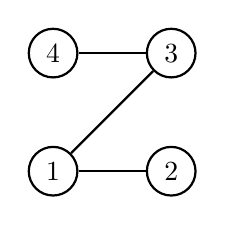
\begin{tikzpicture}[node distance={15mm}, thick, main/.style = {draw, circle}]
        \centering
        \node[main] (1)              {1}; 
        \node[main] (2) [right of=1] {2};
        \node[main] (3) [above of=2] {3}; 
        \node[main] (4) [left of=3] {4};
        \draw  (1) edge (3); 
        \draw  (1) edge (2); 
        \draw  (3) edge (4); 
    \end{tikzpicture}

\end{document}
